\documentclass[12pt,a4paper]{report}

\usepackage[backend=biber, style=ieee]{biblatex}
\addbibresource{literature.bib}

\usepackage[utf8]{inputenc}
\usepackage[T1]{fontenc}
\usepackage[ngerman]{babel}
\usepackage{lmodern}
\usepackage{enumitem}
\usepackage{graphicx}
\usepackage{tabularx}
\usepackage{float}
\usepackage[onehalfspacing]{setspace}
\usepackage{microtype}
\usepackage{parskip}

\usepackage{xcolor}
\newcommand{\todo}[1]{\colorbox{red}{\textbf{TODO: #1}}\\}
\newcommand{\question}[1]{\colorbox{yellow}{\textbf{QUESTION: #1}}\\}
\newcommand{\xeno}[1]{\colorbox{pink}{\textbf{TODO XENO: #1}}\\}
\newcommand{\gideon}[1]{\colorbox{green}{\textbf{TODO GIDEON: #1}}\\}

\begin{document}

\tableofcontents
\newpage


\chapter{Implementierung}

Dieses Kapitel beschreibt die technische Umsetzung der im Konzeptteil definierten Erweiterungen der Yappi-Plattform. Ziel der 
Implementierung war es, die im Rahmen der Produktziele Z-1 bis Z-3 formulierten Anforderungen umzusetzen und die notwendige
Systemarchitektur entsprechend zu erweitern. Die Umsetzung erfolgte unter Berücksichtigung bestehender Komponenten von Yappi, um
eine nahtlose Integration in die vorhandene Codebasis und Betriebsumgebung zu gewährleisten.

Im Folgenden werden die einzelnen Erweiterungen detailliert beschrieben. Beginnend bei der Anpassung der Backend- und
Datenbankstrukturen, über die Entwicklung der Companion-Anwendungen (IntelliJ-Plugin, Kalender-Integration, Health-Companion) bis
hin zur Sicherstellung der Datenübertragung und -sicherheit. Abschliessend werden die getroffenen Entscheidungen hinsichtlich
Deployment und CI/CD-Prozess erläutert, um die vollständige Betriebsfähigkeit der erweiterten Plattform nachzuvollziehen.

Als Grundlage für alle weiteren Erweiterungen wurde Yappi zunächst zu einer Integrationsplattform ausgebaut. Die dafür geschaffene
Integrationsarchitektur bildet den Ausgangspunkt der folgenden Unterkapitel.

\section{Yappi als Integrationsplattform}

Die Erweiterung von Yappi zu einer Integrationsplattform ist notwendig, um Daten aus unterschiedlichen Quellen sicher und 
zuverlässig zu erfassen. Neben Prozessdaten wie Commits oder Meeting-Aktivitäten sollen auch Gesundheitsdaten aus externen
Companion Apps einbezogen werden. Dies erfordert eine Architektur, welche den Datenaustausch zwischen Yappi und externen Anwendungen
standardisiert und absichert. Zentrales Element ist ein API-Key-basiertes Authentifizierungsverfahren, das autorisierte Anwendungen
eindeutig identifiziert und deren Zugriff kontrolliert. Auf dieser Basis können Daten aus heterogenen Quellen in ein einheitliches
System integriert werden.

\subsection{Kommunikationsmechanismus: API-Keys}

Für die Kommunikation zwischen Companion-Anwendungen und dem Yappi Backend wurde bewusst auf einen API-Key-basierten Mechanismus
gesetzt, anstatt die bestehende JWT-basierte Authentifizierung des Frontends zu verwenden. JWTs eignen sich vor allem für die
Authentifizierung einzelner Nutzer in interaktiven Sitzungen. Sie erfordern in der Regel eine vorgelagerte Benutzeranmeldung und
regelmässige Token-Erneuerung. Dieser Ablauf ist für Companion-Anwendungen, die im Hintergrund oder automatisiert Daten erfassen
und übertragen, nicht optimal. Diese würden durch die Notwendigkeit einer manuellen Anmeldung in ihrer Funktionalität eingeschränkt.

Der API-Key-Mechanismus wurde entwickelt, um diesen Anforderungen gerecht zu werden. Jeder Nutzer verfügt über einen persönlichen
API-Key, der in der Webanwendung einmalig generiert wird. Dieser Schlüssel wird manuell in den gewünschten Companion-Anwendungen
hinterlegt. Bei jeder Anfrage an das Backend wird der API-Key im HTTP-Header übermittelt. Das Backend prüft die Gültigkeit des 
Schlüssels und ordnet die Anfrage dem entsprechenden Nutzerkonto zu. So wird sichergestellt, dass nur autorisierte Clients im
Namen des Nutzers Daten übermitteln können. API-Keys lassen sich bei Bedarf widerrufen oder rotieren. Durch diesen Mechanismus
können Companion-Anwendungen zuverlässig und ohne Benutzerinteraktion mit Yappi kommunizieren, während gleichzeitig ein hohes Mass
an Sicherheit gewährleistet ist.

Durch diesen Mechanismus können Companion-Anwendungen zuverlässig und ohne wiederkehrende Benutzerinteraktion mit Yappi 
kommunizieren, während gleichzeitig ein hohes Mass an Sicherheit gewährleistet ist.

\subsection{Systemarchitektur der Integrationsplattform}

\begin{figure}[!htbp]
  \centering
  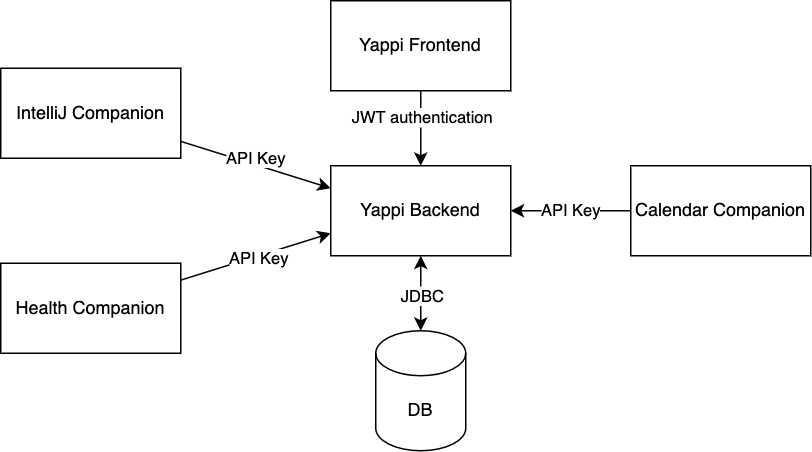
\includegraphics[width=0.95\textwidth]{../figures/plattform-system-diagram.drawio.png}
  \caption{Systemarchitektur der Yappi-Integrationsplattform}
  \label{fig:systemarchitektur}
\end{figure}

Das in Abbildung \ref{fig:systemarchitektur} dargestellte Architekturdiagramm zeigt die zentralen Komponenten der 
Yappi-Integrationsplattform sowie deren Anbindung an externe Companion-Anwendungen. Im Zentrum befindet sich das Yappi Backend,
das als zentrale Schnittstelle für alle eingehenden Daten und Anfragen fungiert.

Das Yappi Frontend verwendet die bestehende JWT-basierte Authentifizierung zur Verwaltung von Nutzersitzungen. Externe
Companion-Apps, wie beispielsweise die IntelliJ-, Health- oder Calendar-Companion, sind über den API-Key-Mechanismus angebunden.
Dieser gewährleistet, dass nur registrierte und autorisierte Clients Daten an das System übermitteln können. Alle eingehenden
Daten werden vom Backend in der dargestellten Datenbank (DB) persistiert.

\subsection{Zugriffskontrolle über API-Keys}

Das API-Key-System dient der sicheren und eindeutigen Authentifizierung externer Dienste gegenüber der \texttt{Yappi-Companion}-API.
Anstelle von Benutzeranmeldedaten verwenden Clients einen statisch generierten API-Key, der für den jeweiligen Nutzer erstellt und ausschliesslich diesem zugeordnet ist.
Dies ermöglicht den kontrollierten Zugriff auf geschützte Endpunkte, ohne dass sensible Login-Daten offengelegt oder dauerhaft gespeichert werden müssen.

Über einen gültigen API-Key können autorisierte Clients Anfragen an Endpunkte mit dem Pfadpräfix \texttt{/companion/} stellen.
Beispielsweise kann der Fragenblock mit der ID~\texttt{1} wie folgt abgerufen werden:

\begin{verbatim}
    GET https://yappi.dev/companion/questionblocks/1
    X-API-KEY: <api-key>
\end{verbatim}

\subsubsection{Backend-Komponenten}

Die Architektur der API-Key-Verwaltung im Backend ist in Abbildung~\ref{fig:apikey-class} dargestellt.  
Das Klassendiagramm zeigt die zentralen Komponenten und ihre Beziehungen, die für die Erstellung, Verwaltung und Validierung von API-Keys erforderlich sind.  
Auf Grundlage dieser Struktur wurde das Backend um die folgenden Elemente erweitert:

\begin{figure}[H]
  \centering
  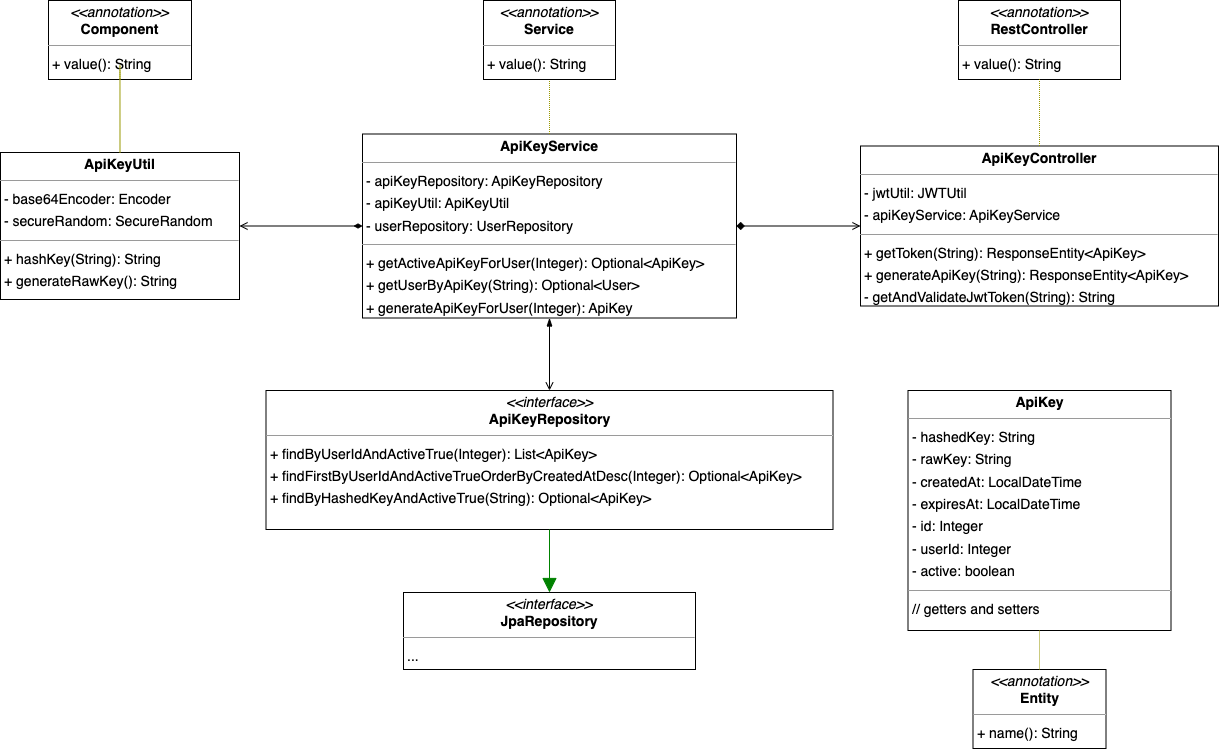
\includegraphics[width=0.95\textwidth]{../figures/apikey-class-diagram.drawio.png}
  \caption{Klassendiagramm für die Implementierung der API-Keys}
  \label{fig:apikey-class}
\end{figure}

\begin{itemize}
  \item \textbf{Entität} (\texttt{ApiKey.java}):  Abbildung der Tabelle \texttt{api\_key} als JPA-Entität.
  \item \textbf{Repository} (\texttt{ApiKeyRepository.java}): Datenbankzugriff auf API-Key-Datensätze.
  \item \textbf{Util-Klasse} (\texttt{ApiKeyUtil.java}): Generierung zufälliger Keys, Hashing mit einem sicheren Algorithmus.
  \item \textbf{Service} (\texttt{ApiKeyService.java}): Erstellung, Speicherung und Validierung von Keys.
  \item \textbf{Controller} (\texttt{ApiKeyController.java}): REST-Endpunkte zur Verwaltung von Keys.
\end{itemize}

\subsubsection{Datenbank Erweiterung}
Das Datenmodell wurde um Die Tabelle~\ref{tab:api_key_schema} \texttt{api\_key} erweitert. Diese speichert die Metadaten und
API-Keys.

\begin{table}[!htbp]
\centering
\begin{tabular}{|l|l|p{9cm}|}
\hline
  \textbf{Spalte} & \textbf{Datentyp} & \textbf{Beschreibung} \\
\hline
  \texttt{id} & SERIAL & Primärschlüssel, auto-inkrementierend \\
  \texttt{user\_id} & INTEGER & Fremdschlüssel auf \texttt{users.id} \\
  \texttt{hashed\_key} & TEXT & Gesalteter Hash des API-Keys \\
  \texttt{raw\_key} & TEXT & Roher API-Key \\
  \texttt{created\_at} & TIMESTAMPTZ & Zeitpunkt der Erstellung des Keys \\
  \texttt{expires\_at} & TIMESTAMPTZ & Ablaufdatum des Keys \\
  \texttt{active} & BOOLEAN & Flag, um Keys ohne Löschung zu sperren \\
\hline
\end{tabular}
\caption{Schema der Tabelle \texttt{api\_key}}
\label{tab:api_key_schema}
\end{table}

Die Speicherung des rohen API-Keys (\texttt{raw\_key}) dient ausschliesslich dem Zweck, diesen dem Benutzer nach der Erstellung 
erneut anzeigen zu können. Diese Entscheidung stellt einen bewussten Kompromiss zwischen Benutzerfreundlichkeit und Sicherheit
dar, wurde jedoch so umgesetzt, dass das Feld bei Bedarf ohne tiefgreifende Änderungen am System entfernt werden kann.

\subsection{Sicherheit}

Der API-Key-Mechanismus der Integrationsplattform ist so konzipiert, dass er eine sichere und kontrollierte Anbindung externer
Companion-Anwendungen ermöglicht. Jeder API-Key ist eindeutig einem Nutzerkonto zugeordnet und wird in der Webanwendung einmalig
generiert. Die Generierung erfolgt über eine abgesicherte Benutzeroberfläche, wodurch sichergestellt ist, dass ausschliesslich
berechtigte Nutzer einen Schlüssel anlegen können. Zur Übertragungssicherheit wird der API-Key ausschliesslich über verschlüsselte
Verbindungen (HTTPS) zwischen der Companion-Anwendung und dem Backend übertragen.

Im Backend erfolgt eine serverseitige Validierung, bei der der Schlüssel auf Gültigkeit und Zuordnung geprüft wird. Die Schlüssel
werden dabei nicht im Klartext gespeichert, sondern in sicherer Form (z. B. gehasht) abgelegt, um auch bei einem möglichen
Datenbankzugriff unbefugten Gebrauch zu verhindern. Ein kompromittierter API-Key kann jederzeit durch den Nutzer oder einen
Administrator gesperrt oder durch einen neuen ersetzt werden.

Die technische Umsetzung der API-Key-Prüfung erfolgt über speziell in Spring Security integrierte Komponenten. Diese sorgen dafür,
dass API-Key-Anfragen noch vor der regulären Benutzer-Authentifizierung ausgewertet und ggf. blockiert werden:

\begin{itemize}
  \item \textbf{ApiKeyFilter} - Spring-Security-Filter, der den API-Key aus dem \texttt{X-API-KEY}-Header ausliest und validiert.
  \item \textbf{SecurityConfig} - Bindet den Filter vor dem \texttt{UsernamePasswordAuthenticationFilter} in die Filterkette ein,
    um API-Key-Anfragen vor anderen Authentifizierungsmethoden zu prüfen.
\end{itemize}

Dieser Prüfmechanismus wird ausschliesslich auf Endpunkten angewendet, deren Pfad den Bestandteil \texttt{/companion} enthält, 
sodass nur für Integrationen mit externen Companion-Anwendungen eine API-Key-Authentifizierung erforderlich ist.

\subsection{Ablauf der API-Key Erstellung und -Verwendung}

Abbildung \ref{fig:apikey-swimlane} zeigt den Ablauf der Erstellung und Verwendung des API-Keys innerhalb der
Yappi-Integrationsplattform. Die Darstellung erfolgt als Swimlane-Diagramm und verdeutlicht die beteiligten Akteure sowie deren
Interaktionen während des gesamten Prozesses.

\begin{figure}[!htbp]
  \centering
  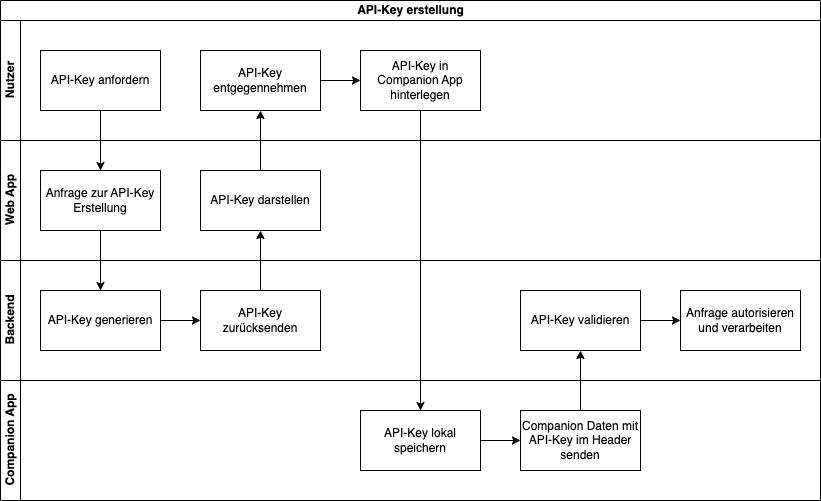
\includegraphics[width=0.95\textwidth]{../figures/apikey-swimlane-diagram.drawio.png}
  \caption{Ablauf der API-Key Erstellung und -Verwendung in Yappi}
  \label{fig:apikey-swimlane}
\end{figure}

Der Prozess beginnt mit der einmaligen Generierung des API-Keys durch den Nutzer in der Webanwendung. Nach der Erstellung wird der
Schlüssel in der Companion-App hinterlegt und dort dauerhaft gespeichert. Jede Datenanfrage der Companion-App an das Backend
enthält den API-Key im HTTP-Header, woraufhin das Backend den Schlüssel validiert und die Anfrage bei positiver Prüfung
autorisiert. Dieser Ablauf stellt sicher, dass ausschliesslich autorisierte Anwendungen im Namen eines Nutzers Daten an Yappi
übermitteln können.

\subsubsection{API-Endpunkte zur API-Key Generierung}

Um einen API-Key über die Webapplikation zu erstellen stehen die folgenden Endpunkte zur verfügung.

Diese Endpunkte setzen einen gültigen JWT im \texttt{Authorization}-Header voraus (\texttt{Bearer <token>}) und sind somit nur 
über das Yappi Frontend erreichbar.

\begin{itemize}
  \item \texttt{GET /apikey} \\
        Liefert den aktiven API-Key des aktuell authentisierten Nutzers. \\
        \textbf{Antworten:} \texttt{200 OK}, \texttt{404 Not Found}, \texttt{401 Unauthorized} (fehlender/ungültiger Header).
  \item \texttt{POST /apikey/generate} \\
        Erzeugt einen neuen API-Key für den authentisierten Nutzer und gibt den API-Key zurück. \\
        \textbf{Antworten:} \texttt{200 OK}, \texttt{401 Unauthorized}.
\end{itemize}

\subsection{Benutzeroberfläche zur API-Key-Verwaltung}

Die API-Key-Verwaltung wurde im Frontend in den Benutzereinstellungen integriert, um Companion-Anwendungen schnell und
unkompliziert mit Yappi verbinden zu können. Die Benutzeroberfläche ermöglicht es, vorhandene API-Keys einzusehen, neue Keys zu
generieren und diese für die weitere Nutzung bequem zu exportieren.  

\begin{figure}[H]
  \centering
  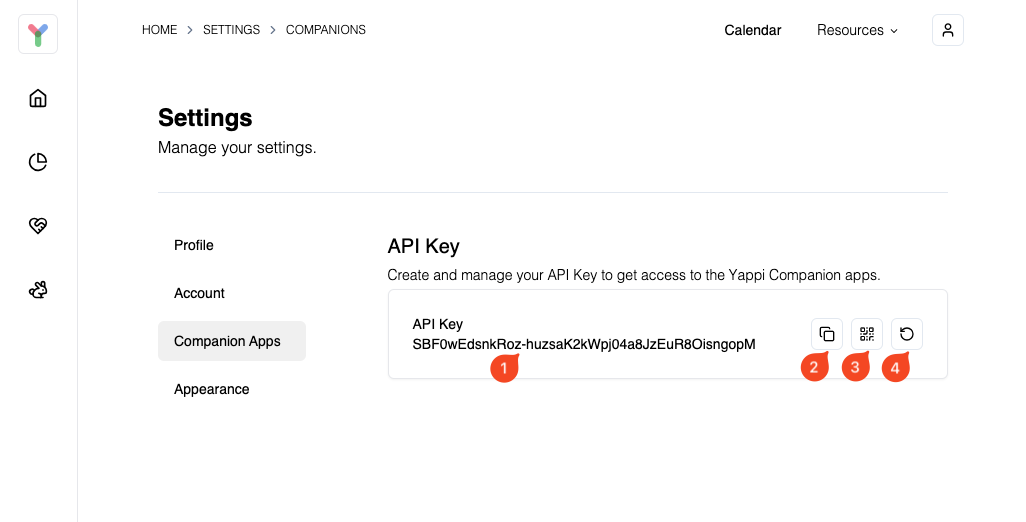
\includegraphics[width=0.95\textwidth]{../figures/yappi-settings-apikey.jpg}
  \caption{Benutzeroberfläche für die Verwaltung von API-Keys im Frontend}
  \label{fig:apikey-frontend}
\end{figure}

Abbildung~\ref{fig:apikey-frontend} zeigt die zentralen Elemente und Funktionen der Implementierung im Frontend:

\begin{enumerate}
  \item \textbf{API-Key-Anzeige}: Zeigt den aktuell gültigen API-Key an.
  \item \textbf{Kopierfunktion}: Kopiert den API-Key in die Zwischenablage, um ihn in Companion-Anwendungen einzufügen.
  \item \textbf{QR-Code-Anzeige}: Zeigt den API-Key als QR-Code an, um ihn mit der mobilen Health Companion App zu scannen.
  \item \textbf{Rotation des API-Keys}: Erzeugt einen neuen API-Key und deaktiviert den bisherigen Schlüssel sofort.
\end{enumerate}


\printbibliography

\end{document}
